\documentclass[11pt,a4paper]{article}
\usepackage[utf8]{inputenc}
\usepackage{amsmath}
\usepackage{amsfonts}
\usepackage{amssymb}
\usepackage{graphicx}
\usepackage{float}
\usepackage{url}
\usepackage{amsmath}
\usepackage{amsthm}
\usepackage{tikz}
\usepackage{amssymb}
\usepackage[french,english]{babel}
\usepackage[french]{cleveref}
\usepackage{svg}
\usepackage{caption}

\usepackage[left=3cm,right=3cm,top=3cm,bottom=3cm]{geometry}

\newtheorem{thm}{Theorem}
\newtheorem{prop}{Propriété}

\theoremstyle{definition}
\newtheorem{defn}{Définition}

\theoremstyle{remark}
\newtheorem{rmq}{Remarque}

\theoremstyle{remark}
\newtheorem{ex}{Exemple}

\usepackage{tikz}
\usepackage{amsmath}

\usetikzlibrary{decorations.pathmorphing, positioning}

\definecolor{echoreg}{HTML}{2cb1e1}
\definecolor{echodrk}{HTML}{0099cc}

\tikzstyle{mybox} = [text=black, very thick,
    rectangle, rounded corners, inner sep=10pt, inner ysep=20pt]
\tikzstyle{fancytitle} =[text=black]

\newcommand{\yslant}{0.5}
\newcommand{\xslant}{-0.6}


\newcommand\overmat[3]{%
  \makebox[0pt][l]{$\smash{\color{#3}\overbrace{\phantom{%
    \begin{matrix}#2\end{matrix}}}^{\text{#1}}}$}#2}
\newcommand\undermat[3]{%
  \makebox[0pt][l]{$\smash{\color{#3}\underbrace{\phantom{%
    \begin{matrix}#2\end{matrix}}}_{\text{#1}}}$}#2}
\newcommand\partialphantom{\vphantom{\frac{\partial e_{P,M}}{\partial w_{1,1}}}}

\author{Pimprenelle Parmentier}



\title{Stream graphes multicouches}
\begin{document}
\selectlanguage{french}
\begin{titlepage}


\noindent
\textsc{Ecole polytechnique}\\
PROMOTION X2016 \\
MASTER: Mathématiques appliquées\\
PARMENTIER Pimprenelle

\vspace{3cm}
\begin{center}
\textsc{\Large Rapport de stage}
\vspace{1cm}
\hrule % Horizontal line
\vspace{0.4cm}
{\huge \bfseries Stream graphes multicouches \par}\vspace{0.4cm} % Thesis title
\hrule 
\vspace{1cm}
\textsc{\Large Rapport non confidentiel}
\vspace{4cm} % Horizontal line
 
\end{center}

\noindent
\textit{Option:} Département de Mathématiques appliquées\\
\textit{Champ:} Etude de graphes\\
\textit{Enseignant référent:} Xavier ALLAMIGEON\\
\textit{Tuteur de stage dans l'organisme:} Tiphaine VIARD\\
\textit {Co-tuteurs de stage hors organisme:} Benjamin RENOUST (Université d'Osaka)\\
\hspace*{6.1cm} Jean-François Baffier (JSPS)\\
\textit{Dates du stage:} 8 avril 2019 - 23 aout 2019\\
\textit{Adresse de l'organisme:}\\
RIKEN AIP\\
Nihonbashi 1-chome Mitsui,\\
Building, 15th floor,\\
1-4-1 Nihonbashi,\\
Chuo-ku, Tokyo\\
103-0027, Japan\\
\end{titlepage}


\begin{abstract}

	


\end{abstract}

\selectlanguage{english}

\begin{abstract}

\end{abstract}

\selectlanguage{french}
\newpage 

\tableofcontents
\newpage



\section*{Introduction}
	Le concept de graphe remonterait à Euler \cite{wikigraphes,divin} dans les années 1750, et s'est révélé extrêmement puissant pour résoudre de nombreux problèmes en algorithmique, probabilités, en combinatoire, en optimisation et plus récemment pour traiter des données.
	La théorie des graphes permet d'exprimer de nombreux problèmes réels dans un même formalisme pour lequel des algorithmes ont été créés.
	
	La théorie des graphes est utilisée dans de nombreux domaines, que ce soit en informatique (analyse de réseaux sociaux, PageRanking \cite{pr}), en biologie, ou dans l'étude des transports par exemple.
	
	Cependant, une partie de l'information est alors perdue, notamment le fait que les interactions entre différents individus dépendent souvent du temps. On "lisse" volontairement les différences au sein des noeuds et des liens, mais une fois encore, on simplifie beaucoup la représentations de nos données.
	
	Notre objectif ici est, en partant de formalismes déjà construits, de créer un nouvel objet nous permettant de représenter des graphes dépendant du temps et prenant en compte les différences au sein des noeuds et des liens. Dans une première partie, nous établirons un état de l'art en rappelant les définitions des graphes, des graphes multicouches et des stream graphes, nous donnerons une bibliographie associée et une analyse critique de ces formalismes. Ensuite, nous présenterons notre nouvel objet, le \og stream graphe multicouche \fg , les définitions associées.
	Nous présenterons enfin la bibliothèque que nous avons créée pour étudier les stream graph multicouche ainsi que quelques exemples de bases de données pour lesquelles il est judicieux d'utiliser notre outil et les résultats que nous avons obtenus sur ces bases. 
	
	
	
\section{Etat de l'art : analyse de deux formalismes sur les graphes}
\indent



Les graphes s'écrivent sous la forme $G=(V,E)$ et servent à modéliser des interactions (arêtes : ensemble $E$) entre des entités (nœuds: ensemble $V$). 

\begin{figure}[H]
	\centering
	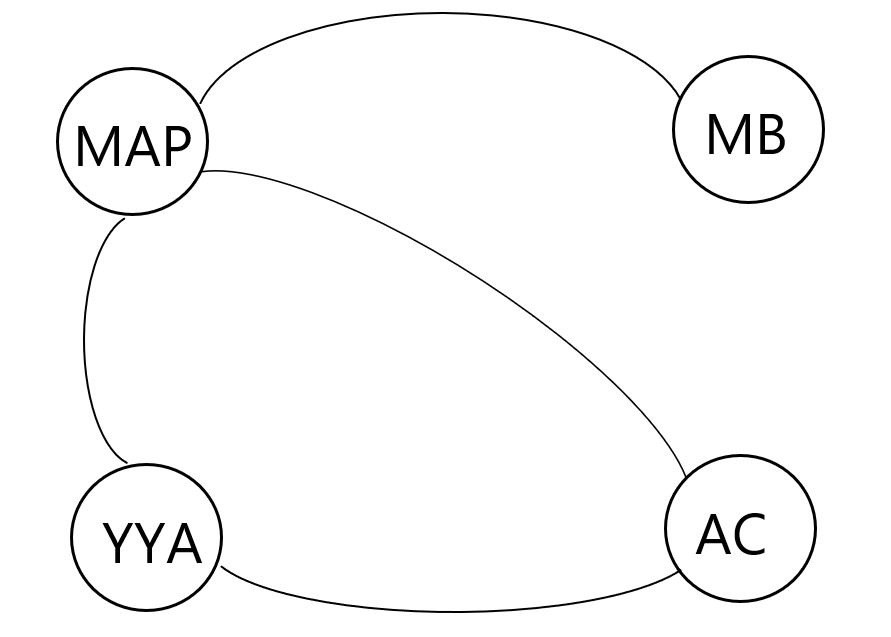
\includegraphics[width=0.3\textwidth]{exGraphe.JPG}
	\caption{Un exemple de graphe de connaissances. Les chercheurs MAP, AC et YYA se connaissent, les chercheurs MB et MAP aussi. En revanche, il n'y a pas de lien entre MB et AC, qui ne se connaissent donc pas.}
\end{figure}


\subsection{Les graphes multicouches}

\subsubsection{Définition générale}

 Les graphes multicouches sont utilisés pour décrire des interactions entre des noeuds qui peuvent être de différentes natures de façon simultanée et/ou qui peuvent avoir des interactions de natures différentes. 
 
 Une définition très générale des graphes multicouches est donnée dans le papier \cite{mlkiv}, nous la résumons ici.
 
 La structure d'un graphe multicouches est décrite par le k-uplet d'ensembles ${\cal L} = L_1, \dots , L_k$. Chaque $L_i$ est un ensemble d'attributs que peut avoir une couche, appelés "couches élémentaires". Chaque couche correspond donc à un élément de $L=L_1\times L_2 \times \dots \times L_k$.
 
 Un graphe multicouches s'écrit alors $M = (V_M, E_M, V, L)$. $V$ est l'ensemble de ses noeuds, $L$ la structure des couches, $V_M$ sont les noeuds-couches, qui comme leur nom l'indique, sont les éléments de $V\times L$. Enfin $E_M \subseteq V_M \times V_M $ est l'ensemble des liens, un lien pouvant relier deux noeuds-couches entre eux. 
 
 On peut trouver un exemple de graphe multicouche \cref{exmulti}.

\begin{figure}[h]
	\centering
	
%0.58
\begin{tikzpicture}[scale=0.38,every node/.style={minimum size=1cm},on grid]

	\node [mybox, scale=1.0] at (10.5, 2) (box){%
		\begin{minipage}{0.6\textwidth}
			
    	\end{minipage}
	};
	
	
	% etage 2
	\begin{scope}[
		yshift=-210,
		every node/.append style={yslant=\yslant,xslant=\xslant},
		yslant=\yslant,xslant=\xslant
	] 
		%\draw[black, dashed, thin] (0,0) rectangle (7,7); 
		\fill[olive,fill opacity=.75] (0,0) rectangle (7,7);
		
		\fill[orange,fill opacity=.75] (10,0) rectangle (17,7);
		%\draw[black, dashed, thin] (10,0) rectangle (17,7); 
		
		\draw[fill=echoreg]  %foret, collabo
			(5,2) node(111){} circle (.1) %A
			(2,2) circle (.1) %B
			(2,5) circle (.1); %C
			%(5,5) circle (.1); %D
		
		\draw[fill=echoreg]  %plaine, collabo
			(15,2) node(111){} circle (.1) %A
			%(12,2) circle (.1) %B
			(12,5) circle (.1) %C
			(15,5) circle (.1); %D
		 
		\draw[ thin, color=echodrk]%foret collab
			(2,4.9) to (2,2.1); %C->B
		\draw[ thin, color=echodrk]
			(2.1,2) to (4.9,2);%B->A
		
		\draw[thin, color=echodrk]%plaine collab
			(12,5) to (15,2);%C->A
		\draw[thin, color=echodrk]
			(12,5) to (15,5);
			
		\fill[black]
			(0.5,6.5) node[right, scale=.7] {Forêt, Collaboration}	
			(5.1,1.9) node[right,scale=.7]{\bf A}
			(1.9,1.9) node[left,scale=.7]{\bf B}
			(2,5.2) node[left,scale=.7]{\bf C};
			%(5.2,5.1) node[right,scale=.7]{\bf D}; 
			
		\fill[black]
			(10.5,6.5) node[right, scale=.7] {Plaine, Collaboration}	
			(15.1,1.9) node[right,scale=.7]{\bf A}
			%(11.9,1.9) node[left,scale=.7]{\bf B}
			(12,5.2) node[left,scale=.7]{\bf C}
			(15.2,5.1) node[right,scale=.7]{\bf D}; 
		
		
	\end{scope}
	
	% Interlayer crossconnections
	% vertical
	\draw[thick,  dashed, decorate] (3.8, 4) to (3.8, -3.5);%A
	\draw[thick, dashed, decorate] (.8,2.4) to (.8,-5);%B
	\draw[thick,  dashed, decorate] (-1, 4.5) to (-1, -2.8);%C
	
1	\draw[thick,  dashed, decorate] (13.8,9) to (13.8, 1.5);%A
	\draw[thick, dashed, decorate] (12,11) to (12,3.6);%D
	\draw[thick,  dashed, decorate] (9, 9.5) to (9, 2.1);%c
	
	%horizontal
	
	
	\draw[thick, dashed, decorate] (-1,-2.8) to[bend left] (9,2.1);
	\draw[thick, dashed, decorate] (3.8,-3.5) to[bend left] (13.8,1.5);
	
	
	% etage 1
	\begin{scope}[
		yshift=0,
		every node/.append style={yslant=\yslant,xslant=\xslant},
		yslant=\yslant,xslant=\xslant
	]
		\fill[olive,fill opacity=.85] (0,0) rectangle (7,7); 
		%\draw[black, dashed, thin] (0,0) rectangle (7,7); 
		
		\fill[orange,fill opacity=.85] (10,0) rectangle (17,7);
		%\draw[black, dashed, thin] (10,0) rectangle (17,7); 
		
		\draw [fill=red]
			(5,2) node(111){} circle (.1)%A %foret, combat
			(2,2) circle (.1)%B
			(2,5) circle (.1)%C
			(5,5) circle (.1);%D

		\draw[fill=red]  
			(15,2) node(111){} circle (.1) %A % plaine combat
			%(12,2) circle (.1) %B
			(12,5) circle (.1) %C
			(15,5) circle (.1); %D
		
		\draw[thin, color=red]%foret combat
			(2,2.1) to (2,4.9);%B->C
			
		\draw[thin, color=red]%plaine combat
			(12,5) to (15,5);%C->D
		
		
		\fill[black]
			(0.5,6.5) node[right, scale=.7] {Forêt, Combat}
			(5.1,1.9) node[right,scale=.7]{\bf A}
			(1.9,1.9) node[left,scale=.7]{\bf B}
			(1.9,5) node[left,scale=.7]{\bf C}
			(5.2,5.1) node[right,scale=.7]{\bf D}; 
			
		\fill[black]
			(10.5,6.5) node[right, scale=.7] {Plaine, Combat}
			(15.1,1.9) node[right,scale=.7]{\bf A}
			%(11.9,1.9) node[left,scale=.7]{\bf B}
			(12,5.2) node[left,scale=.7]{\bf C}
			(15.2,5.1) node[right,scale=.7]{\bf D};
			
	\end{scope} 
	
	%interlayer
	\draw[thick, dashed, decorate] (-1,4.5) to[bend left] (9,9.5);
	\draw[thick, dashed, decorate] (3.8,4) to[bend left] (13.8,9);
	\draw[thick, dashed, decorate] (2.1,6.1) to[bend left] (12,11);
\end{tikzpicture}

	\caption{\textbf{Représentation d'un graphe multicouches.} Ici, les noeuds sont des animaux d'une même espèce représentés par leurs initiales: $V = \{A ,B,C,D \}$. Chaque couche est caractérisée par une milieu naturel et un type de relation: $L = \{$Milieu, type de relation$\}$. Les noeuds couches existent ou non en fonction de la présence ou non d'un animal dans un milieu pour un type de relation: $V_M$ contient par exemple (A;Forêt,Combat). Enfin, les liens représentent les interaction entre les animaux dans un milieu précises: $E_M$ contient par exemple ((B;Forêt,Collaboration),(C;Forêt, Collaboration)).}
	\label{exmulti}
\end{figure}

\subsubsection{Cadres d'utilisation}


Les graphes multicouches trouvent de nombreuses applications, par exemple en \textbf{écologie} \cite{ecolo} (les noeuds sont alors des espèces ou des individus, les couches élémentaires des types d'interaction (parasite, prédateur...), des lieux, des temps, etc. On cherche alors à savoir comment se diffuse une maladie, quelles sont les faiblesses d'un écosystèmes (quels sont les liens / nœuds qui assurent le bon fonctionnement ?)

Un autre jeu de données utilisé est en \textbf{économie}, celui des interactions entre les banques européennes \cite{interbank}, les couches étant caractérisées par le type d'interaction (de "prêt"), les noeuds étant les banques et un lien existant entre deux banques de la même couche quand celles-ci procèdent à une interaction du type correspondant.

Un dernier exemple intuitif est celui des \textbf{réseaux de transport}, dans lequel les couches sont les différents moyens de transport possible, les nœuds sont des localités et les liens les différentes lignes de transport. Un tel jeu de données peut être trouvé sur le site gouvernemental américain des statistiques de transport, pour les lignes aériennes \cite{plane}.

On remarque que dans beaucoup de situations, nous avons des liens "implicites" entre tous les différents noeuds-couches issus du même noeud, et des liens "explicites" ne pouvant apparaitre qu'au sein d'une même couche. De tels graphes sont appelés \textbf{multiplexes}.





%Ils permettent de représenter des graphes de collaboration entre chercheurs par exemple : chaque chercheur collabore avec d'autres sur des mots-cles précis, les noeuds sont alors les chercheurs, les couches les différents mots-clés utilisés et des liens apparaissent entre deux chercheurs-mots clés quand les deux chercheurs apparaissent sur le même papier traitant du mot-clé.

\subsubsection{Quelques définitions}

\begin{defn}{\textbf{Tenseur d'adjacence}}
	
\end{defn}
D'un point de vue pratique, ces graphes peuvent être manipulés à l'aide de tenseurs d'adjacence \cite{mldd}, d'ordre 4. Chaque élément $M^{u,\alpha}_{v,\beta}$ indique s'il existe un lien entre les nœuds-couches $(u,\alpha)$ et $(v,\beta)$.

\begin{defn}{\textbf{Arêtes intra-couches et inter-couches.}}
	On appelle arêtes inter-couches les arêtes qui lient deux nœud-couches de couches différentes. (L'ensemble des arêtes inter-couches s'écrit $E_A = \{((u,\alpha),(v,\beta)) \in E_M | \alpha = \beta\}$). On appelle arêtes intra-couches les arêtes qui lient deux noeuds-couches de la même couche. (L'ensemble correspondant s'écrit $E_C = E_M\backslash E_A$).
\end{defn}
Ainsi, les multiplexes sont des graphes multicouches dans lesquels les seuls arêtes intercouches autorisées sont les arêtes entre les noeuds-couches du même noeud.

\begin{defn}{\textbf{Graphe agrégé}}
	On appelle le graphe aggrégé le graphe qu'on obtient en "superposant" les couches d'un graphe multicouches : $$G=(V_G,E_G), \quad V_G=V, \quad E_G={(u,v)|\exists \alpha, \beta | ((u,\alpha),(v,\beta)) \in E_M}$$.
\end{defn}

\begin{defn}{\textbf{Graphe sous-jacent}}
Le graphe sous-jacent de $M$ est le graphe qu'on obtient en faisant abstraction de la structure multicouches, et dans lequel chaque noeud est un noeud-couche.
$$G=(V_{SJ},E_{SJ}), \quad V_{SJ} = V_M, \quad E_{SJ}=E_M$$
\end{defn}




\subsubsection{Pourquoi utiliser des graphes multicouches à la place de graphes classiques ?}

On remarque que dans beaucoup de cas, les graphes sont des graphes agrégés ou sous-jacent de graphes multicouches. Une partie de l'information a été "perdue" mais cela permet d'utiliser des outils très puissants et d'obtenir des résultats déjà satisfaisants grâce à la théorie des graphes. On peut donc se demander quel est l'intérêt d'utiliser ce formalisme, et de garder une telle quantité d'informations. De nouvelles mesures et de nouveaux algorithmes ont donc été créés pour pouvoir analyser plus finement ces informations plus détaillées.

En voici deux exemple, qui seront source d'inspiration dans la suite sur ce qu'il sera possible de faire avec l'objet que nous allons introduire.


\paragraph{Importance de la structure : Isomorphismes de graphes}

Deux graphes $G_1$ et $G_2$ sont dits isomorphes quand on peut trouver une bijection des sommets du premier graphes vers ceux du second qui préserve les arêtes.


\begin{figure}[H]
\centering
	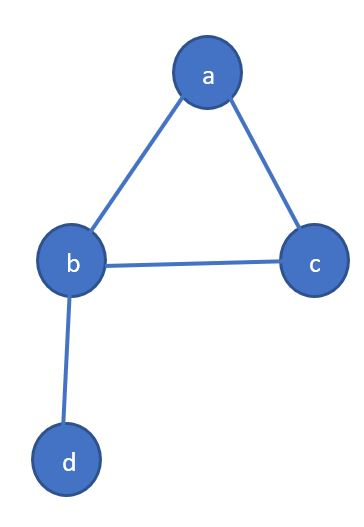
\includegraphics[width=0.2\textwidth]{graph1iso.JPG}
	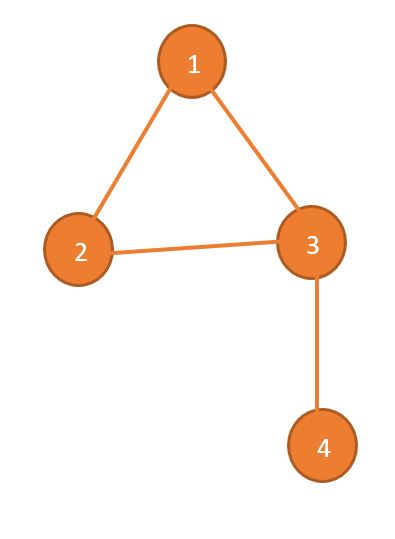
\includegraphics[width=0.2\textwidth]{graph2iso.JPG} 
	
	\caption{Un exemple de deux graphes isomorphes : $\sigma(a)=1, \sigma(b)=3, \sigma(c)=2, \sigma(d)=4$}
\end{figure}

Dans le cadre des multicouches, Kivelä et Porter \cite{isoMulti} définissent l'automorphisme de graphe (sans perte de généralité) par une permutation des arêtes, des couches élémentaires et des couches qui préserve les liens.


Kiveä et Porter démontrent qu'il n'est pas équivalent de dire que deux graphes multicouches sont isomorphes et leurs graphes sous-jacent sont équivalents. En effet, il ne faut pas perdre de vue que la structure "arborescente" des couches, doit être conservée, et pas seulement l'idée de "partition" des nœuds en différentes couches. Ils présentent un algorithme permettant de vérifier si deux graphes multicouches sont isomorphes.

\paragraph{Centralité}

La question de la centralité a été traitée dans \cite{centraliteMulti}. De Domenico met en avant le fait qu'il est "réducteur" de calculer des centralités sur des graphes agrégés pour trouver quels sont les noeuds ayant les roles les plus centraux dans la cohésion de l'ensemble d'une structure. Ils définissent donc un nouveau "PageRank" et une nouvelle centralité intermédiaire (betweeness centrality). Le PageRank est calculé à partir du tenseur d'adjacence du graphe, on obtient alors des centralités pour chaque noeud-couche, qu'on traite de la manière la plus adaptée en fonction du problème à résoudre.

La centralité intermédiaire est calculée en sommant les centralités intermédiaires des différents nœuds-couches.

De Domenico montre que le fait de conserver l'information multicouche permet de trouver un classement des noeuds en fonction de leur centralité plus proche de la réalité (il compare ses résultat avec des données réelles sur les aéroports par exemple).

\paragraph{}

Nous avons présenté ici deux exemples pour lesquels il a été judicieux de conserver l'aspect mutlicouche des graphes, parce qu'il contient plus d'informations, et qu'elles ont une structure particulière.


\subsection{Les stream graphs}



Les stream graphs ont été créés dans le but de pouvoir mieux étudier les graphes dynamiques, c'est à dire des graphes dont les nœuds et les liens peuvent apparaitre et disparaitre au fil du temps.

\subsubsection{Définition}

\begin{defn}{\textbf{Stream graph}}
Un stream graph s'écrit $S=(T,W,V,E)$. $T$ représente l'intervalle de temps d'étude de notre graphe. $V$ est l'ensemble des nœuds, et $W \subseteq T \times V$ est l'ensemble des nœuds de $V$ apparaissant en fonction du temps. Enfin, $E \subseteq T \times V \times V$ est l'ensemble des liens dont l'existence dépend également du temps. Étant donné un noeud $u$, on appelle $T_u$ l'union des intervalles pendant lesquels $u$ apparait, de même que $T_{u,v}$ décrit les temps d'apparition du lien $(u,v)$.
\end{defn}

La représentation graphique des stream graphes est une des grandes forces du concept et permet de visualiser l'évolution des graphes au fil du temps.

\begin{figure}[H]
\centering
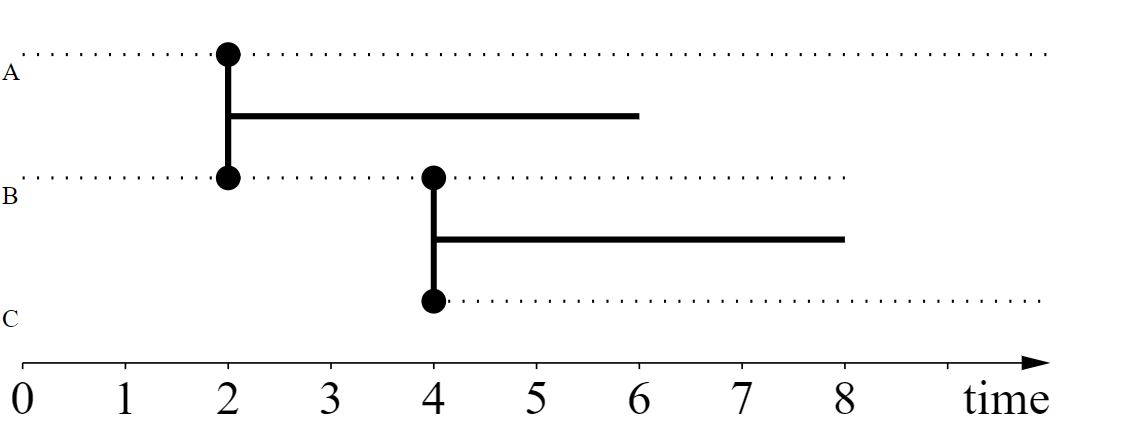
\includegraphics[width=0.5\textwidth]{exStreamGraph.JPG}
\caption{\textbf{Exemple de stream graph.} Dans cet exemple, on représente les interactions entre chercheurs durant une conférence de 10 heures ($T=[0,10]$). Les nœuds sont les trois chercheurs ($V=($MAP,MB,YYA$)$) et leurs intervalles d'existence sont les suivants $T_{\text{MAP}}=[4,10], T_{\text{MB}}=[0,10], T_{\text{YYA}}=[0,8]$, ils représente les moments où les chercheurs étaient présents à la conférence. Enfin les liens $V=([2,6]\times (\text{MB},\text{YYA})) \cup ([4,8]\times(\text{YYA},\text{MAP}))$ représentent les moments où les chercheurs ont discuté entre eux.}
\end{figure}




\subsubsection{Quelques définitions}

Dans l'article \cite{stream}, de nombreuses notions sont ensuite définies de telle sorte à ce que dans le cas où le stream graph serait statique, on retrouve les mêmes notions que pour un graphe classique.

Nous les évoquerons en temps voulu quand nous nous en servirons pour créer nos propres définitions.

\subsubsection{De l'intérêt de l'usage des stream graphs}
La notion de stream graphe est très récente (2017)\cite{stream} et ce n'est évidemment pas la première tentative de formalisme pour des graphes dynamiques.

Par exemple on peut citer la représentation souvent utilisée en recherche opérationnelle, en "snapshot". Le nombre de noeuds d'un système est multiplié par un nombre de pas de temps discrets $n=\frac{t}{T}$. On crée ensuite un graphe temporel dont les noeuds sont étiquetés $(v,t_i)$, $v$ étant les noeuds et $t_i$ les temps auxquels ils sont considérés. Les liens peuvent être présents entre différents noeuds du même pas de temps, et on ajoute à cela une arête entre tous les couples de noeuds de la forme $(v,t_i),(v,t_{i+1})$. 
Dans ces cas-là les liens sont très souvent orientés pour indiquer le sens du temps. Ces graphes sont utilisés pour des calculs de flots optimaux \cite{map}. On peut d'ailleurs raccrocher cette représentation à la théorie des graphes multicouches, chaque couche correspondant à un pas de temps.

La notion de stream graph permet de "se libérer" de la vision discrétisée des snapshots. Même si dans l'absolu, les deux visions permettent de stocker les mêmes informations et de faire les mêmes choses (il suffit pour cela de choisir un pas de discrétisation assez petit), la vision stream graph permet d'aborder le problème sous un autre angle, plus orienté sur l'étude des ensembles d'intervalles qui caractérisent les liens et les nœuds.

\begin{figure}
\centering
	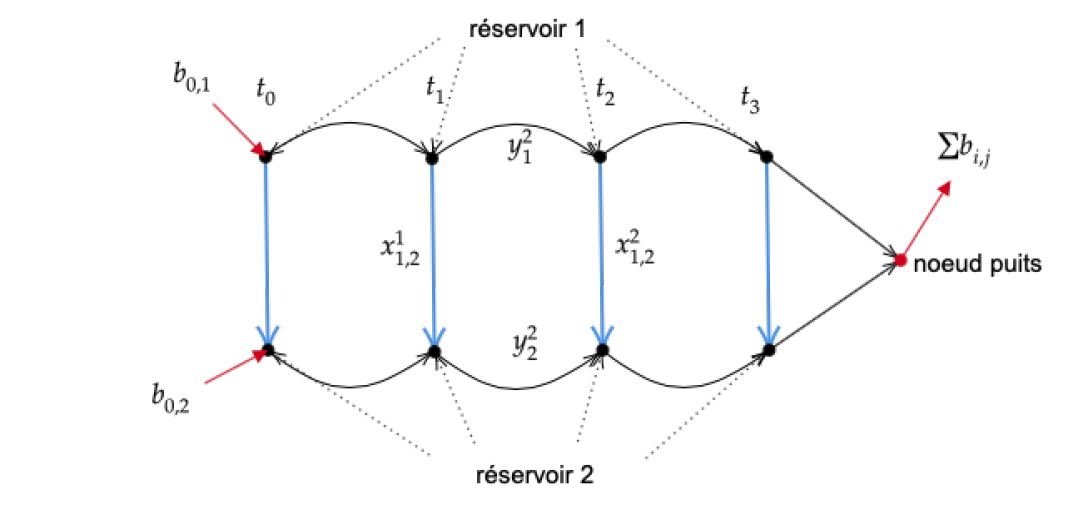
\includegraphics[width=0.7\textwidth]{snapshot.JPG}
	\caption{\textbf{Exemple de snapshot:} Un "snapshot" représentant un barrage (liens bleus) entre deux réservoirs aux temps $t_0,t_1,t_2,t_3$, tiré d'un projet MAP552}
\end{figure}



%conclusion partielle : cohérence avec les graphes classiques, à l'utilisateur de choisir ce qu'il veut obtenir

 
\section{Présentation d'un nouvel objet: le stream graph multicouche}



\subsection{Motivations}
\subsection{Définition}

\begin{defn}[\textbf{Stream graph multicouche}]
    
    Soit $T$ un intervalle de temps, ${\cal L}$ une structure de couches définie comme dans le cadre des graphes multicouches simples, et $V$ un ensemble de noeuds. 
    
    $T_M$ est un ensemble d'intervalles inclus dans $T$, indexé par les couches de $L$ et représente le temps d'existence de ces couches, avec pour contrainte que $\cup_{\alpha \in L} T_{\alpha} = T$ . $W_M$ est inclus dans $T \times V \times L$, et contient les temps d'existence de chaque nœud couche, sachant que le temps d'existence d'un nœud couche est forcément inclus dans le temps d'existence de la couche. Enfin, $E_M \subseteq T \times V \times L \times V \times L$ donne les liens entre les nœuds couches et leurs temps d'existence, sachant qu'un lien ne peut exister que pendant l'intersection des temps d'existence des nœuds-couches qu'il relie.
    
    L'objet $S_M = (T,T_M,V,W_M,E_M,{\cal L})$ est alors appelé \textbf{stream graph multicouches } (ou multilayer stream graph en anglais).
    
    On définit également les temps d'existence des noeuds-couches $T_{u,\alpha}$ et les temps d'existence des liens $T_{(u,\alpha),(v,\beta)}$ qui sont des unions d'intervalles.
	\end{defn}
	
	\begin{figure}[H]
		\centering
		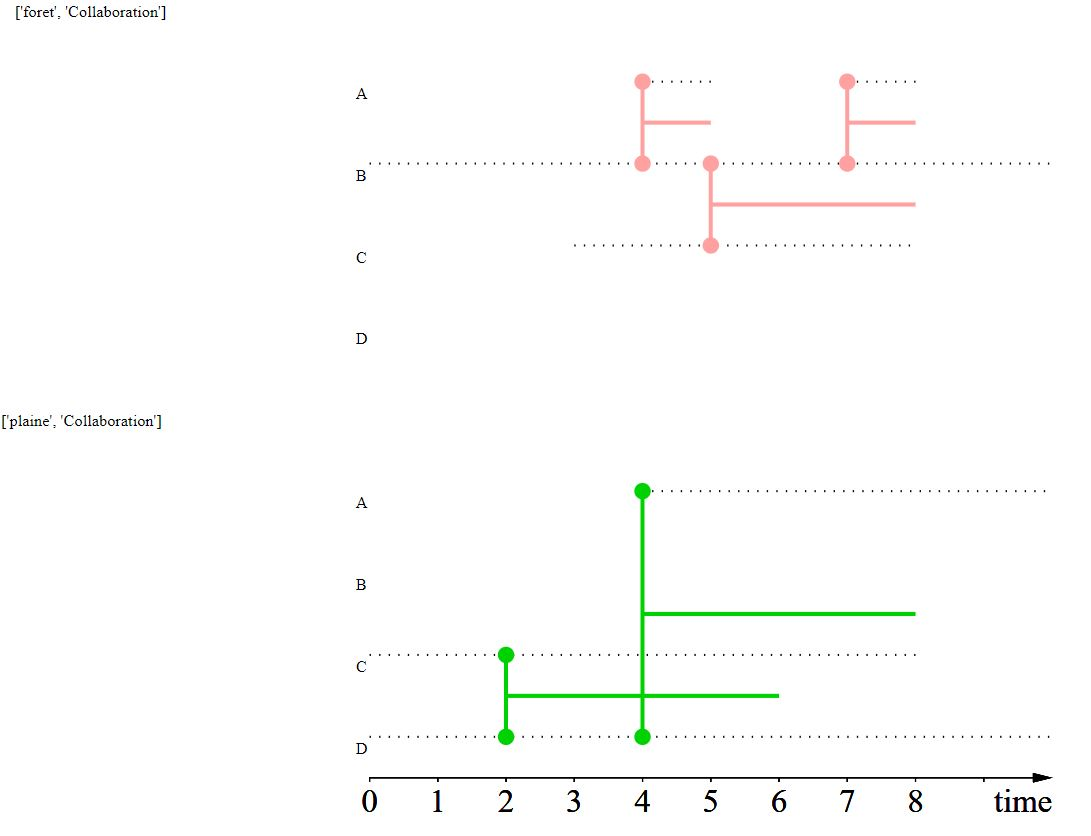
\includegraphics[width=0.8\textwidth]{exMultiStream.JPG}
		\caption{La représentation en multilayer stream graph des couches ["ECCS13","Talk to each other"] et ["Workshop in Oxford","Talk to each other"], générée avec "multiplex-stream" (description du programme en partie \cref{descode})}
	\end{figure}
	
	\begin{rmq}
		On peut s'interroger sur le bien-fondé d'utiliser l'objet stream graph pour rajouter l'aspect temporel aux graphes multicouches. En effet, dans \cite{mlkiv}, les auteurs évoquent l'idée d'un aspect "continu", pouvant représenter le temps. Mais cette idée ne semble pas avoir été beaucoup exploitée, car les outils développés pour manipuler les graphes multicouches sont principalement matriciels et donc faits pour traiter un nombre de couches fini. De plus, des outils ont été spécifiquement créés pour traiter les stream graphs et l'idée ici est de les exploiter.
	
	\end{rmq}

\subsection{Extraction de sous-graphes}
\label{sousgraphes}
\subsubsection{Projection par rapport au temps}
	Nous définissons ici deux moyens d'extraire des graphes multicouches en s'affranchissant du temps.
	
	Le premier est de "prendre une photo" au temps $t$ :
	\begin{defn}[Graphe multicouche au temps t]
   	Le {\em graphe multicouche au temps t} $M_t$ s'écrit $M_t = (V_{M,t}, E_{M,t},V,{\cal L})$ avec $V_{M,t}$ et $E_{M,t}$ contenant les noeuds-couches et les arrêtes apparaissant au temps $t$.
   	$$ V_{M,t} = \{ (u,\alpha) | (t,u,\alpha) \in W_M\} $$
   	$$ E_{M,t} = \{(u,\alpha,v,\beta) | (t,u,\alpha,v,\beta) \in E_M\}$$

   \end{defn}

	\begin{figure}[h]
		\begin{minipage}{0.49\linewidth}
			%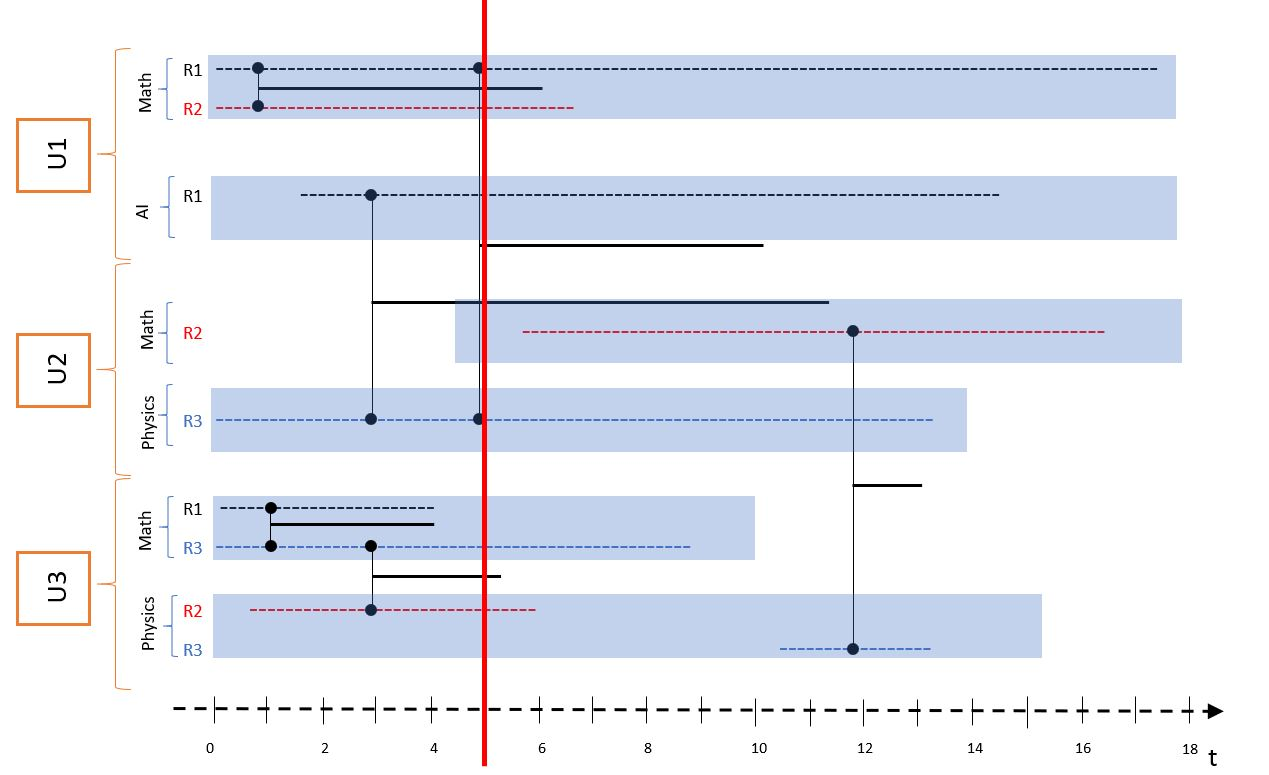
\includegraphics[width=\textwidth]{schemas/pauset.jpg}
		\end{minipage}
		\begin{minipage}{0.49\linewidth}
			%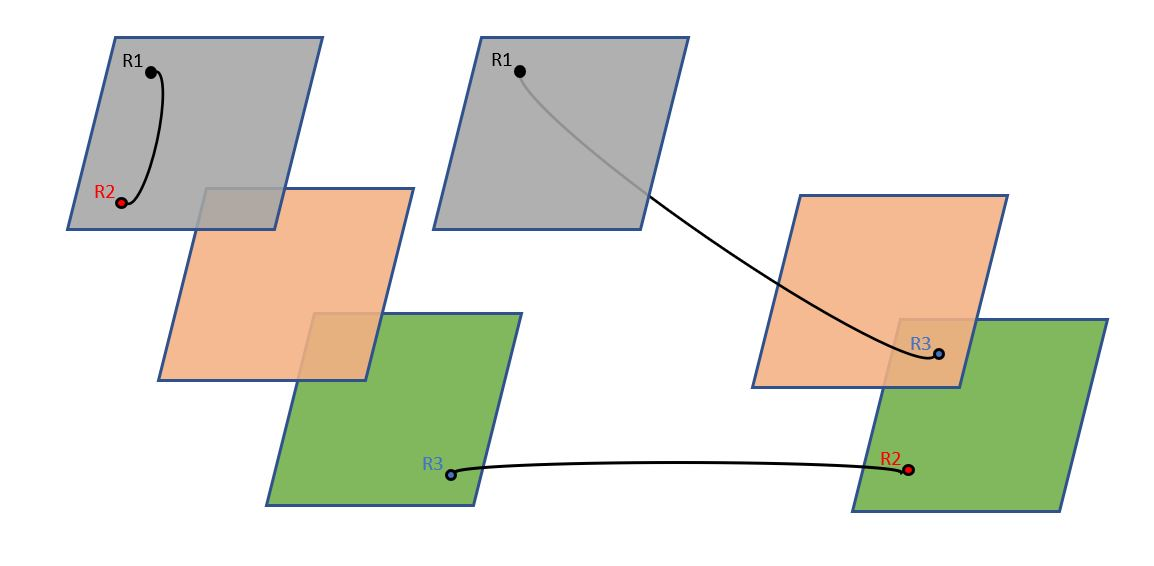
\includegraphics[width=\textwidth]{schemas/pausetproj.jpg}
		\end{minipage}
		\caption{dessin d'une extraction}
	\end{figure}

    
    Le {\em graphe multicouche induit} $M_I(S_M) = (V_{M,I}, E_{M,I}, V,L)$ de $S_M$ est le graphe multicouche qui rassemble toutes les couches, noeuds couches et noeuds qui ont apparu durant $T$.
    \begin{align*}
    	V_{M,I} = \bigcup_{t\in T} V_{M,t}\\
    	E_{M,I} = \bigcup_{t\in T} E_{M,t}\\
    \end{align*}
    
	


\subsubsection{Projection à partir de couches}
Comme dans \cite{mlkiv} pour les graphes multicouches, nous pouvons "classifier" les arêtes en plusieurs catégories :
	
	\begin{defn}[Arêtes de couplage, arêtes intra-couches et inter-couches]

   	Les {\em arêtes de couplage} sont définies par l'ensemble $E_C=\{(t,u,\alpha,v,\beta)\in E_M | u=v\}$.

    Les {\em arêtes intra-couches} sont définies par l'ensemble $E_I = \{(t,u,\alpha,v,\beta) \in E_M | \alpha = \beta \}$

    Les {\em arêtes inter-couches} sont définies par l'ensemble $\bar{E_I} = E_M\backslash E_I$.
    
	%(See fig.\ref{exIntraInter} for a visual representation.)
	
	\end{defn}	
	
	\begin{figure}[h]
		\centering
		%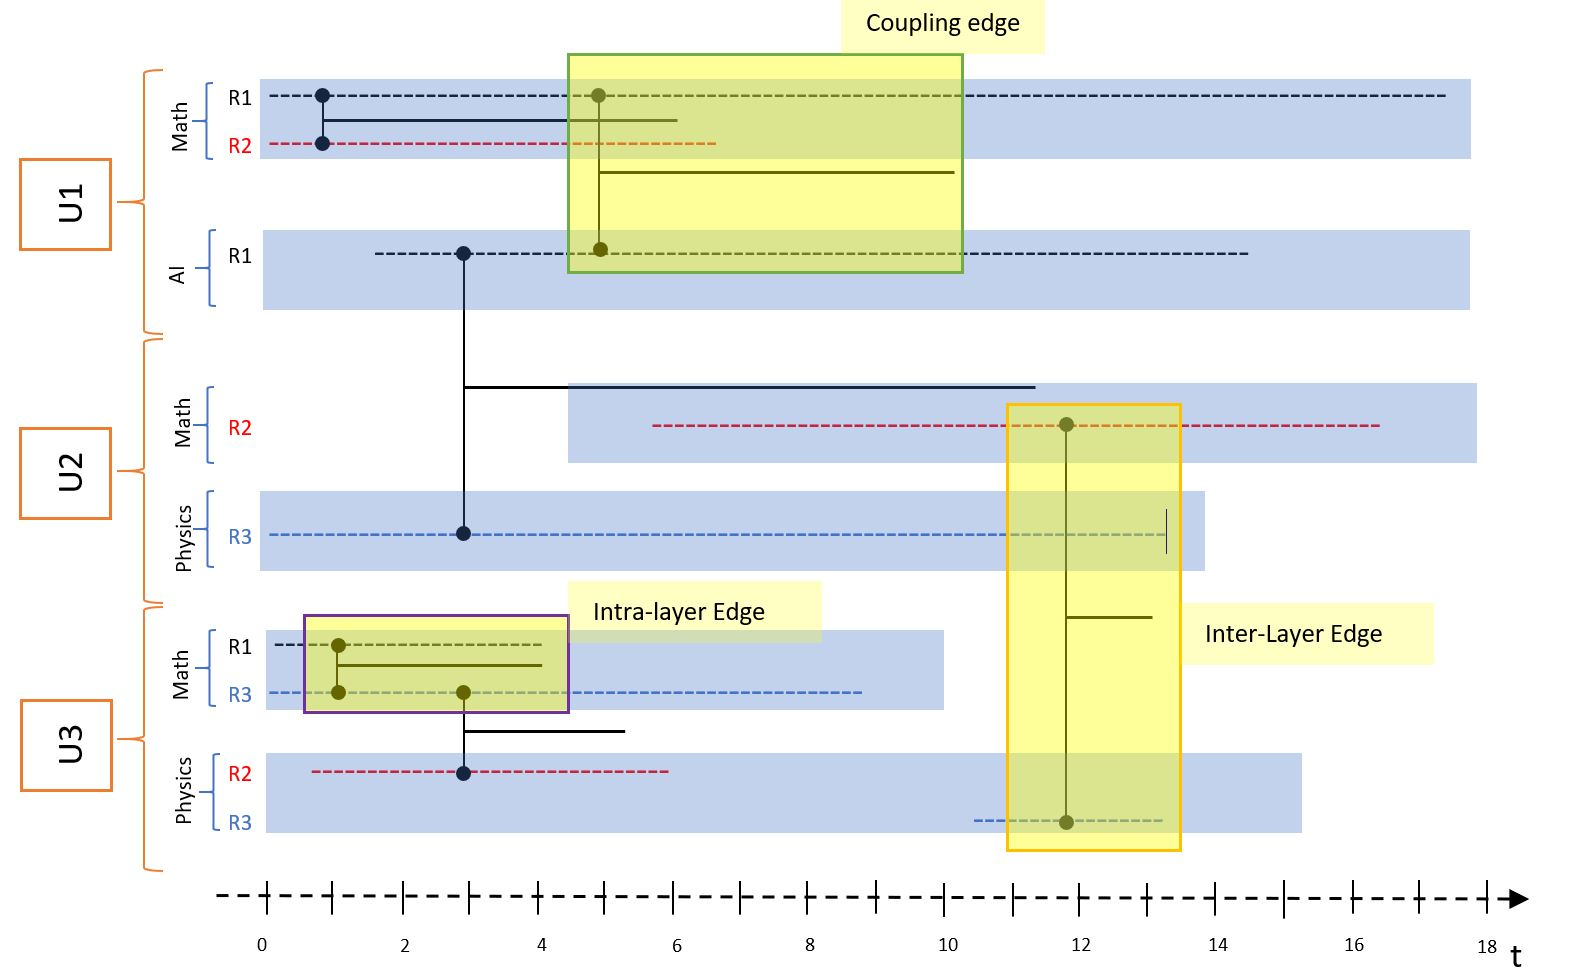
\includegraphics[width=\textwidth]{schemas/edgesCat.jpg}
		\caption{Illustration with our example of coupling edges, intra-layer edges and inter-layer edges}
		\label{exIntraInter}
	\end{figure}
	
	
	Comme dit précédement, les graphes multiplexes sont présents dans beaucoup de cas concrets et font l'objet d'études qui leur sont particulièrement dédiées. Nous définissons ici de façon formelle les stream graphs multiplexes.
	
	\begin{defn}[Stream graph multiplexe]	
	Un {\em stream graph multiplexe} est un graphe dans lequel chaque arête est une arête intra-couche ou une arête de couplage.
	\end{defn}
	
	
	 
	\begin{defn}[Stream graph intra-couche]
	Pour chaque couche $\alpha \in L_1 \times \dots \times L_d$, le {\em stream graph intra-couche} $S^{\alpha}$ est le stream graph $S^{\alpha}=(T^{\alpha},V^{\alpha},W^{\alpha},E^{\alpha})$ tel que $T^{\alpha} = T_{\alpha} \in T_M$ est l'intervalle d'existence de $\alpha$. $V^{\alpha}$ est l'ensemble des nœuds couches dans la couche $\alpha$ et $W^{\alpha}$ représente leurs temps d'apparence dans la couche $\alpha$. $E^{\alpha}$ est le sous-ensemble $E_M$ contenant seulement les arêtes entre les noeuds-couches de $\alpha$.
	\end{defn}
	
	
	\begin{defn}[Stream graph inter-couches]	
	Pour chaque doublet de couches $\alpha, \beta \in L_1\times \dots\times L_d$, le {\em stream graph inter-couches} est le stream graph $S^{(\alpha,\beta)} = (T, V^{\alpha,\beta},W^{\alpha,\beta},E^{\alpha,\beta})$ tel que : $T^{\alpha,\beta}=T^{\alpha}\cap T^{\beta}$ est l'intervalle durant lequel $\alpha$ et $\beta$ apparaissent simultanément. $V^{\alpha,\beta}$ sont tous les noeuds-couches du stream graph multicouche qui sont dans les couches $\alpha$ et $\beta$, $W^{\alpha,\beta}$ décrit leurs intervalles d'existence. Enfin, $E^{\alpha,\beta}$ sont les liens non orientés entre les noeuds couches des couches de $\alpha$ et $\beta$ avec leurs temps d'existence.
	\end{defn}
	
	%english Notice that for any layer $\alpha$,  is equivalent to $S^{(\alpha,\alpha)}$.

	On remarque que pour toute couche $\alpha$, $S^{(\alpha)}$ est équivalent à $S^{(\alpha,\alpha)}$.


	Après avoir extrait les stream graphes d'intérêt, il nous pouvons effectuer des opérations d'union et d'intersection pour trouver des propriétés intéressantes.
	
	\begin{defn}[Intersection de deux stream graphs]
	L'{\em intersection} de deux stream graphs $S_1$ et $S_2$ est un stream graph et est définie de la façon suivante :
	\[
		S' = S_1 \cap S_2 = (T_1\cap T_2, V_1 \cap V_2, W_1 \cap W_2, E_1\cap E_2)
	\]
	\end{defn}
	

	\begin{defn}[Union de deux stream graphs]
	L'{\em union} de deux stream graphs $S_1$ et $S_2$ est un stream graph et est définie de la façon suivante :
	\[
		S' = S_1 \cup S_2 = (T', V_1 \cup V_2, W_1 \cup W_2, E' \})
	\]
	$T'$ est un intervalle :
	\[
		T' = [\min(T_1,T_2),\max(T_1,T_2)]
	\]
	\[
		E' = E_1 \cup E_2 
	\]
	
	\end{defn}
	
	
	\begin{defn}[Underlying stream]
		The {\em underlying stream } $S_U(S_M)$ of $S_M$ is $(T,V_M,W_M,E_M)$. Its is the stream graph in which the nodes are the node-layers. It could be shared into clusters corresponding to the different layers. This definition is a generalisation to the one defined on \cite{mlkiv} for simple multilayer graphs.
	\end{defn}
	
	\begin{defn}[Aggregated stream]
		
		The {\em aggregated stream} $S_A(S_M)$ has the same $T$ as $S_M$. Its nodes are the nodes of $S_M$ and a link exists between two nodes if and only a link exist between two correspondent node-layers.	This definition is a generalisation to the one defined on \cite{mldd} for simple multilayer graphs.
	
	\end{defn}
	
	We can now demonstrate that the underlying stream graph is the union of all the intra and inter layer stream graphs.
	
	\begin{prop}
		\[
			\bigcup_{(\alpha,\beta) \in L^2} S^{(\alpha,\beta)} = S_U(M_S)
		\]
	\end{prop}
	\begin{proof}
	We call $S=\bigcup_{(\alpha,\beta) \in L^2} S^{(\alpha,\beta)}=(T^{*},V^{*},W^{*},E^{*})$ and we want to show that $S=S_U(M_S)=S_U(M) = (T_U,V_U,W_U,E_U)$.
	
	$T=T_U$ by definition of $S_U$. By construction of multilayer stream graphs, at each $t\in T$, at least one layer $\alpha$ is existing. Then as $T* = [\min_{\alpha \in L} (T^{\alpha}),max_{\alpha \in L} (T^{\alpha})]$, $t$ is included in $T*$. Each $T^{\alpha}$ is included in $T$, so $T^* \subseteq T$, which leads us to $T^*=T_U=T$.
	
	$V_M = V_U$ by definition of $V_U$.$V^{*}=\bigcup_{(\alpha,\beta) \in L^2} V^{\alpha,\beta} \subseteq V_M$. All the nodes of all the layers are included in $\bigcup_{(\alpha) \in L^2} V^{\alpha,\alpha} \subseteq V^{*}$, so we obtain the equality $V_M=V_U=V^*$.
	With the same argument we find that $W_M=W_U=W^*$.
	
	$E_U=E_M$ and $E^{*}=\bigcup_{\alpha,\beta \in L^2}(E^{\alpha,\beta})$ by definition. So as $E^{\alpha,\beta}$ is a subset of $E_M$ for every couple of layers $\alpha,\beta$, $E^{*} \subset E_M$. We notice too that for every $e =(t,u,\alpha,v,\beta) \in E_M$, $e$ belongs to $E^{\alpha,\beta}$. So $\mathbf{E_M=E^{*}}$.
					
	\end{proof}

\subsubsection{Remarque sur les extractions}
On remarque que de nombreux graphes et graphes multicouches sont extraits de stream graphs multicouches.


\subsection{Mesures}


Nous avons créé des mesures permettant de mesurer la présence de liens et de nœuds dans les graphes. Nos exigences pour ces mesures sont qu'elles soient adaptées à l'objet spécifique que nous étudions (et qu'elles prennent en compte l'aspect multicouche et l'aspect temporel de façon simultanée), qu'elles aient des noms qui évoquent intuitivement ce qu'elles expriment et qu'elles soient une généralisation des notions utilisées pour les stream graphs, pour les graphes multicouches et pour les graphes.

	\subsubsection{Nombre de nœuds}
	Le {\em nombre de noeuds dans un graphe} $G=(V,E)$ est $|V|$ et le nombre d'arêtes est $|E|$.
	
	Le {\em nombre de noeuds dans un stream graph} $S=(T,V,W,E)$ est défini dans \cite{stream} comme $\hat{N}^T_n=\frac{|W|}{|T|}=\sum_{v\in V} n_v$. $n_v$ est appelé {\em contribution de v} et est égal à $\hat{N}^T_v=\frac{|T_v|}{|T|}$. Remarquons bien qu'ici cette notion est différente {\em du nombre de noeuds dans} $|V|$, sauf quand le stream graphe $S$ est constant au cours du temps.
	\newline
	
	Dans les graphes multicouches, une telle notion n'a pas été définie explicitement.
	Nous avons donc défini le {\em nombre moyen de noeuds par couche} comme :
	\begin{align*}
		\hat{N}_n^L(M_l) = \frac{\text{nombre de noeud-couches}}{\text{nombre de couches}}=\frac{|V_M|}{|L|}
	\end{align*}	    
	Remarquons que dans le cas d'un monocouche, nous retrouvons le nombre de noeuds classique, ce qui signifie que nous pouvons choisir cette mesure comme une généralisation du {\em nombre de nœuds} dans un graphe, comme cela a été fait dans \cite{stream} pour les stream graphs.
		
	
	\begin{defn}[Contribution des couches]
	On définit la {\em contribution} d'une couche comme suit : $n_\alpha = \frac{|T_{\alpha}|}{|T|}$. Le {\em nombre de couche dans un stream graph multicouches} est la somme des contributions. $\hat{N}^T_l = \sum_{\alpha \in L}\frac{ |T_{\alpha}|}{|T|}$.
    \end{defn}
	
	\begin{defn}[Contribution et quantité de nœud-couches]
	La {\em contribution d'un noeud-couche} dans un stream graphe multicouche est $n_{v,\alpha} = \frac{|T_{v,\alpha}|}{|T|}$. Le {\em nombre de nœud-couches} est la somme de leurs contributions $\hat{N}^{T}_{nl}(M) = \underset{(u,\alpha)\in V_M}{\sum} n_{(u,\alpha)} = \frac{|W_M|}{|T|}$.
    \end{defn}
	
	Dans le cas d'un stream monocouche, nous retrouvons bien que le nombre de noeuds est égal au nombre de noeuds-couches. En prenant le stream graph sous-jacent du stream graphe multicouche, on retrouve également que le nombre de noeuds est égal au nombre de noeuds couches. Nous avons donc là une généralisation satisfaisante du nombre de noeuds-couches.
    
   Enfin, nous définissons le \textbf{nombre de noeuds dans un stream graph multicouches} de la façon suivante : 
    
    \begin{defn}[Contribution et nombre de noeuds dans un stream graph multicouche]
    La {\em contribution} d'un noeud décrit le taux d'apparition d'un noeud dans les couches : $n_v = \frac{\sum_{\alpha \in L}|T_{v,\alpha}|}{\sum_{\alpha \in L} |T_{\alpha}|}$.
    
    Le {\em nombre de noeuds} est la somme de ces contributions :
    \begin{align}
    \hat{N}^{L,T}_n(M) = \sum_{v\in V} n_v= \sum_{v\in V} \frac{\sum_{\alpha \in L}|T_{v,\alpha}|}{\sum_{\alpha \in L} |T_{\alpha}|} 
    \label{numberNodes}
	\end{align}     
	
	\end{defn}
	
	Cette définition est cohérente avec les notions des multicouches et des stream graphs : si le noeud apparait dans toutes les couches tout le temps, nous trouvons $n_v=1$ comme dans les multicouches. Si tous les temps d'existence sont égaux, on retrouve $$n_v=\frac{\text{nombre de noeud-couches issus de v}\times |T|}{\text{nombre de couches}\times |T|}$$ Cette définition est donc une bonne généralisation pour tous les concepts.

	


	\subsubsection{Uniformité et densité}
	
	Dans les stream graphs \cite{stream}, {\em l'uniformité entre deux nœuds} $u$ et $v$ est le ratio $\Cup (u,v) = \frac{|T_u\cap T_v|}{|T_u \cup T_v|}$, c'est à dire la probabilité, prenant un temps $t$ dans $T_u$ ou $T_v$, que les deux nœuds $u$ et $v$ puissent être reliés entre eux. L'uniformité est définie comme le rapport de tous les temps de co-existence sur les temps d'existence : $
 \Cup(S)=\sum_{u,v \in V \otimes V}\frac{|T_u\cap T_v|}{|T_u\cup T_v|}
$
	
		
	{\em L'uniformité } de deux noeuds-couches $(u,\alpha)$ et $(v,\beta)$ est définie sur le même modèle :
	\begin{align*}
		\Cup((u,\alpha),(v,\beta))=\mathbb{P}( t \in T_{u,\alpha} \cap T_{v,\beta} | t \in T_{u,\alpha} \cup T_{u,\beta}) \\
		= \frac{|T_{u,\alpha}\cap T_{u,\beta}|}{|T_{u,\alpha}\cup T_{u,\beta}|}
	\end{align*}

	{\em Le chevauchement} de deux couches $\alpha$ et $\beta$ est également défini comme suit :
	\begin{align*}
		\cup(\alpha,\beta) = \frac{|T_{\alpha}\cap T_{\beta}|}{|T_{\alpha}\cup T_{\beta}|}
	\end{align*}

    L'{\em uniformité des noeuds-couches} mesure le taux d'apparition simultanée des noeuds-couches dans le stream-graphe multicouche :
    \[
    	\Cup(M) = \frac{\sum_{(u,\alpha),(v,\beta) \ V_M \otimes V_M}{|T_{(u,\alpha)} \cap T_{(v,\beta)}|}}{\sum_{(u,\alpha),(v,\beta) \ V_M \otimes V_M}{|T_{(u,\alpha)}\cup T_{(v,\beta)}|}}
    \]
	
	Cette définition peut être nuancée en considérant que selon la nature du stream graph multicouche, certains noeuds peuvent ou ne peuvent pas apparaitre simultanément. En particulier, {\em l'uniformité dans un stream graph multiplexe} est définie ainsi:	
	
	\[
    	\Cup(M) = \frac{1}{|L|}\sum_{\alpha \in L} \frac{\sum_{(u,\alpha),(v,\alpha) \ V_M \otimes V_M}{|T_{(u,\alpha)} \cap T_{(v,\alpha)}|}}{\sum_{(u,\alpha),(v,\alpha) \ V_M \otimes V_M}{|T_{(u,\alpha)}\cup T_{(v,\alpha)}|}}
    \]
    
    On ne prend en compte que les temps d'apparition intra-layer, et on moyenne selon le nombre de couche. 


	Quand $\Cup=1$, on dit que le stream graph est uniforme (autrement dit, $T_v = T_u, \forall (u,v) \in V^2$).


    Après avoir mesuré "à quel point le stream graphe multilayer peut être connecté" grâce à l'uniformité, nous allons mesurer à quel point il est effectivement connecté grâce à a notion de \textbf{densité}.
    
    Dans les graphes classiques (non pondérés et non directionnel), la {\em densité} est la probabilité, prenant deux noeuds au hasard dans le graphe, qu'une arête existe entre ces noeuds.
    
		\[
			d(G) = \frac{|E|}{|V\otimes V|} = \frac{2\times |E|}{|V|(|V|-1)}
		\]
	Dans les stream graphs, la notion définie dans \cite{stream} est la même , en prenant un temps et deux noeuds au hasard existant à ce temps. 	

		\begin{align*}
			\delta_s(G) = & \mathbb{P}((t,u,v)\in E| (t,u),(t,v) \in W) \\
			 =  & \frac{\sum_{uv \in V \otimes V}{|T_{uv}|}}{\sum_{uv \in V\otimes V}{|T_u\cap T_v|}}= \frac{\int_{t\in T}{|E_t|dt}}{\int_{t\in T}{|V_t\otimes V_t|dt}}
		\end{align*}
		
	Nous pouvons ensuite définir la densité dans les stream graphs multicouches. Nous remarquons premièrement que la densité mesure le "taux de connectivité", et qu'une fois encore, en fonction du système étudié, la définition peut changer puisque nous voulons que le cas où la densité est égale à 1 corresponde au cas où on ne peut pas rajouter d'arêtes. Nous appelons  $C \in T \times V_M\times V_M$ l'ensemble des connections autorisées dans le stream graphe multicouches. Si certaines connections sont \og automatiques\fg ou "sous-entendues" comme par exemple les connections de couplage, nous ne les comptons pas dans $C$ non plus pour que le cas où la densité soit nulle corresponde au cas où on ne peut pas retirer de lien.


	\[
		\delta_M (M) 
		= \frac{\int_{t\in T}|E_M,t|}{\int_{t\in T}|C_t|} 
		= \frac{\sum_{(u,\alpha)(v,\beta) \in E_M}|T_{(u,\alpha)(v,\beta)}|}{|C|}
	\]

	Par exemple, dans un stream graph multiplexe, les liens possibles sont les liens intra couches et les liens de couplage : $C=\{(t,u,\alpha),(t,v,\beta))| t\in T_{u,\alpha} \cap T_{u,\beta}, u=v \text{or} \alpha = \beta)\}$ :

	\[
		\delta_M (M) = 
		\frac{|E_M|}{|C|}= 
		\frac{\sum_{(u,\alpha)(v,\beta) \in (V_M \otimes V_M)} |T_{(u,\alpha)(v,\beta)}|}
		{\underbrace{(\sum_{\alpha \in L}\sum_{(u,v) \in V\otimes V}|T_{u,\alpha} \cap T_{v,\alpha}|)}_{\text{arêtes intra-couches}}+\underbrace{( \sum_{u \in V } \sum_{(\alpha,\beta) \in L \otimes L}|T_{u,\alpha}\cap T_{u,\beta}|)}_{\text{arêtes de couplage}}}
	\]

	
\section{Application à des données concrètes}

\subsection{Structure de données et organisation du code} 
\label{descode}

	La gestion des flots de liens multicouche implique assez rapidement de gérer un grand nombre d'informations "imbriquées" : chaque couche contient des noeuds, qui apparaissent à des temps précis, ces noeud-couches sont reliés par des liens, eux-mêmes apparaissant à des temps précis...
	
	J'ai choisi de construire des classes python pour simplifier la gestion de telles données, et pour permettre de vérifier simplement que le stream graph multicouche reste cohérent quand on le modifie.
	
	
	
	\begin{figure}[H]
		\centering
		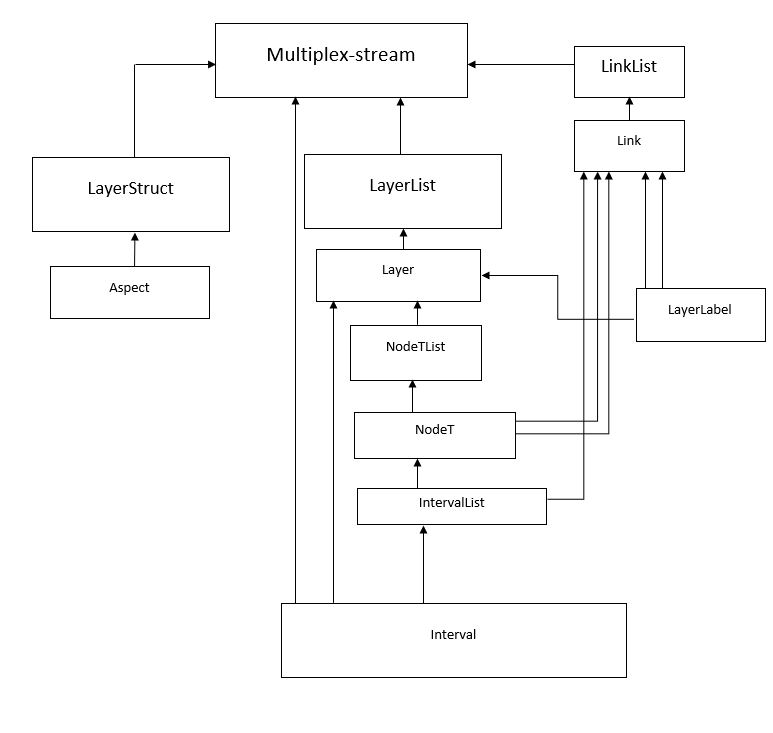
\includegraphics[width=0.5\textwidth]{codeStructure.JPG}
		\caption{Structure du code en classes }
	\end{figure}
	
	Toutes les listes sont toujours triées et les listes d'intervalles contiennent seulement des intervalles disjoints (quitte à fusionner certains intervalles).
	
	

\subsection{CPGE : interactions entre élèves d'un même établissement}

Nous avons en premier lieu testé notre logiciel avec une base de donnée de SocioPatterns (\cite{cpge}), recensant les interactions de "face à face" entre élèves (enregistrées toutes les 20 secondes grâce à des capteurs de proximité), leurs amitiés sur Facebook, le fait qu'ils connaissent leur numéro de téléphone, et leur réponse à un questionnaire leur demandant s'ils étaient amis.

Nous avons donc choisi une structure de multilayer suivante : \\
{\tt L=[type de relation,classe,sexe]},\\
 avec\\
  {\tt type de relation = [face to face, facebook, contact, amitié]},\\
  {\tt classe = "MP","MP*1","MP*2","2BIO1","2BIO2","2BIO3","PSI*","PC","PC*"}.
  
  Le temps de prise a duré 5 jours, les détecteurs s'activant toutes les 20 secondes.
  
  Comme les seules interactions dépendantes du temps sont celles de face à face, on peut dire que le jeu de donnée donne forcément lieu à un graphe "hybride".
  
	\subsubsection{Représentation graphique}  
  
  Nous avons tout d'abord tenté de représenter le graphe multicouche en entier (\cref{lyceeentier}). Sa taille le rend difficile à représenter (d'ailleurs, trouver un ordre optimal pour les noeuds qui limite les croisements des liens est un problème d'optimisation qui n'a pas encore été résolu de façon satisfaisante).
	
	\begin{figure}[h]
	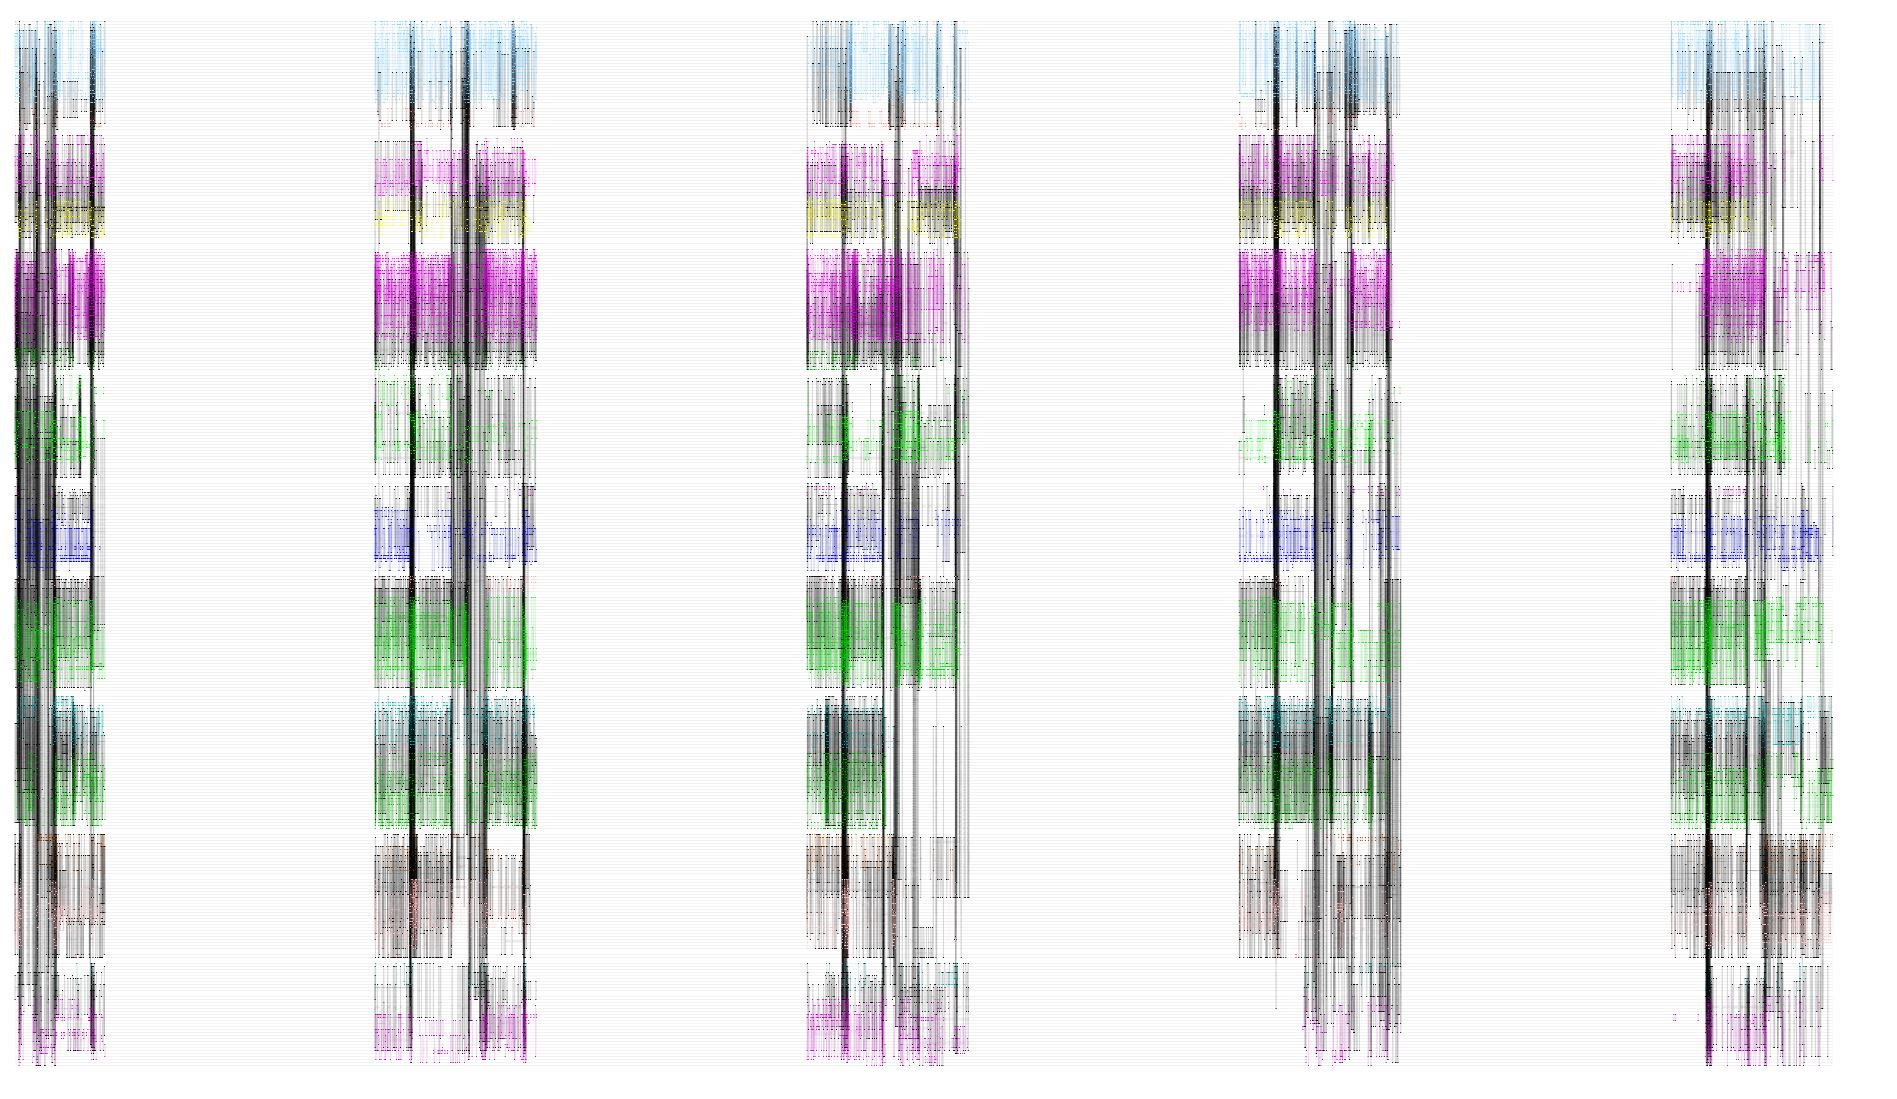
\includegraphics[width=\textwidth]{lyceeentier.JPG}
	\caption{\textbf{Visualisation du stream graphe multilayer du dataset \cite{cpge}.} Les liens intra-couches ont été coloriés dans des couleurs aléatoires. On remarque des apparitions de liens inter-couches assez importants au moment des "pauses" (il y a visiblement une pause le matin, une autre le midi, et à la fin de la journée). On peut également visualiser simplement l'emploi du temps des élèves (représentés par des vides dans le graphe).}
	\label{lyceeentier}
\end{figure}





\subsubsection{Sous-graphes, sous-streams et sous graphes multicouches}

Voici quelques exemples de sous-graphes tels que nous les avons définis \cref{sousgraphes}. Nous avons décidé de nous cantonner aux relations \texttt{'face to face'} et \texttt{'facebook'}, mais ces résultats sont généralisables à plus de couches. 




\paragraph{Graphe induit}
	Le graphe multicouche induit des relations de deux classes, filles et garçons, est représenté \cref{completinduit}.
	
\begin{figure}[h]
	\centering
	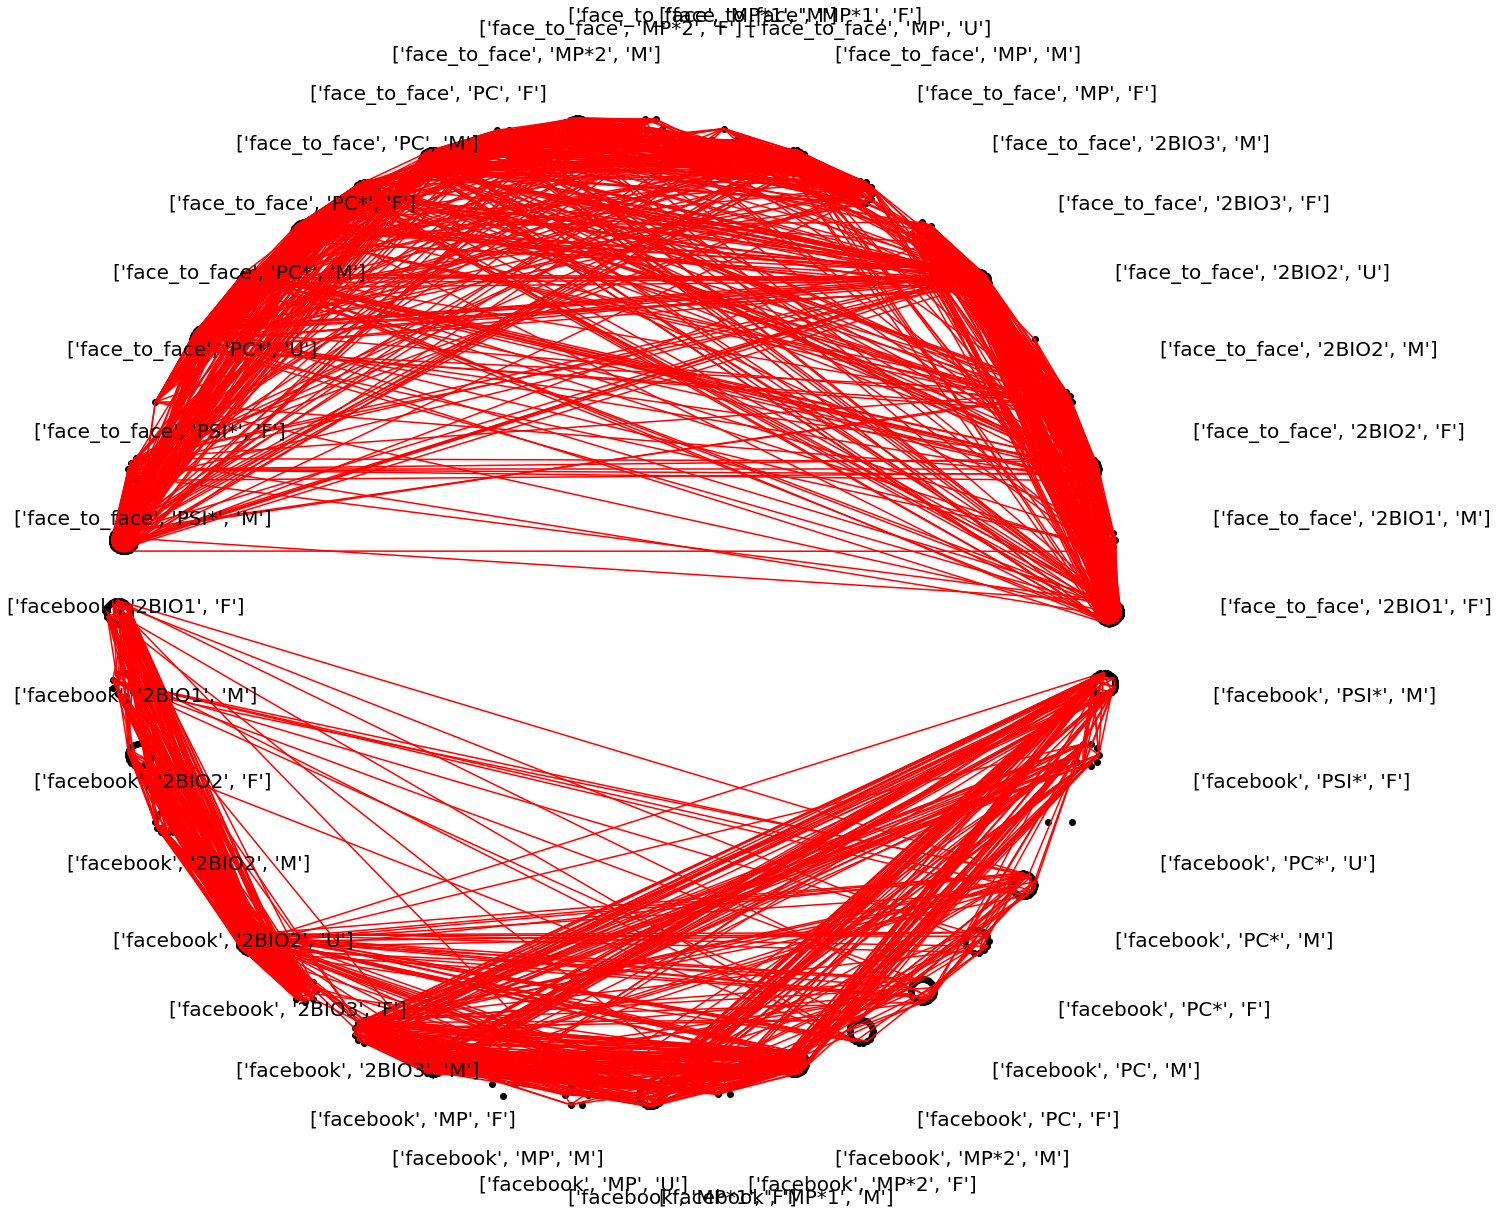
\includegraphics[width=0.5\textwidth]{tout.png}
	\caption{\textbf{Graphe induit}}
	\label{completinduit}
\end{figure}

	Nous représentons ensuite les sous-graphes multicouches intra-couches et inter-couches des couches de deux classes différentes pour plus de visibilité.


	
	On peut alors se demander en regardant le schéma, si la règle "



\begin{figure}[h]
	\begin{minipage}[t]{0.48\textwidth}
		\captionsetup{margin=10pt}
		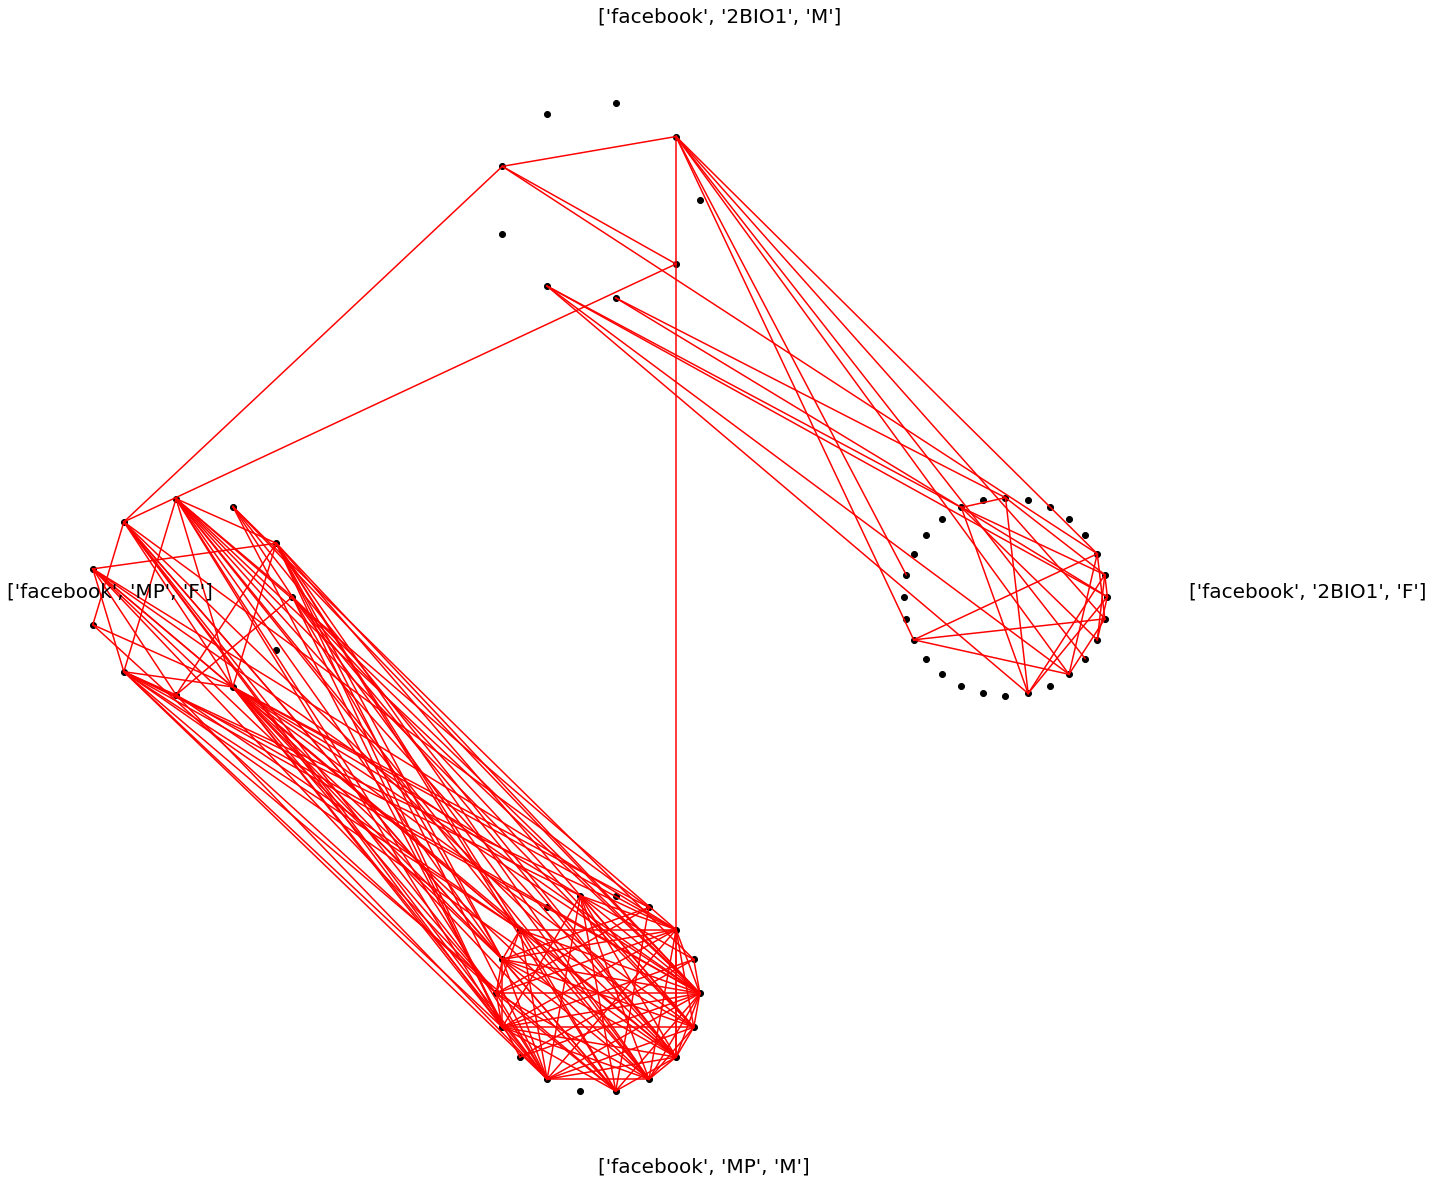
\includegraphics[width=\textwidth]{sousmulticlasse.png}
	\caption{\textbf{Visualisation du sous graphe multicouches des relations \texttt{'facebook'}, entre les élèves de deux classes} : les \texttt{'2BIO1'} et les \texttt{'MP'}.}
	\end{minipage}
	\begin{minipage}[t]{0.48\textwidth}
		\centering
		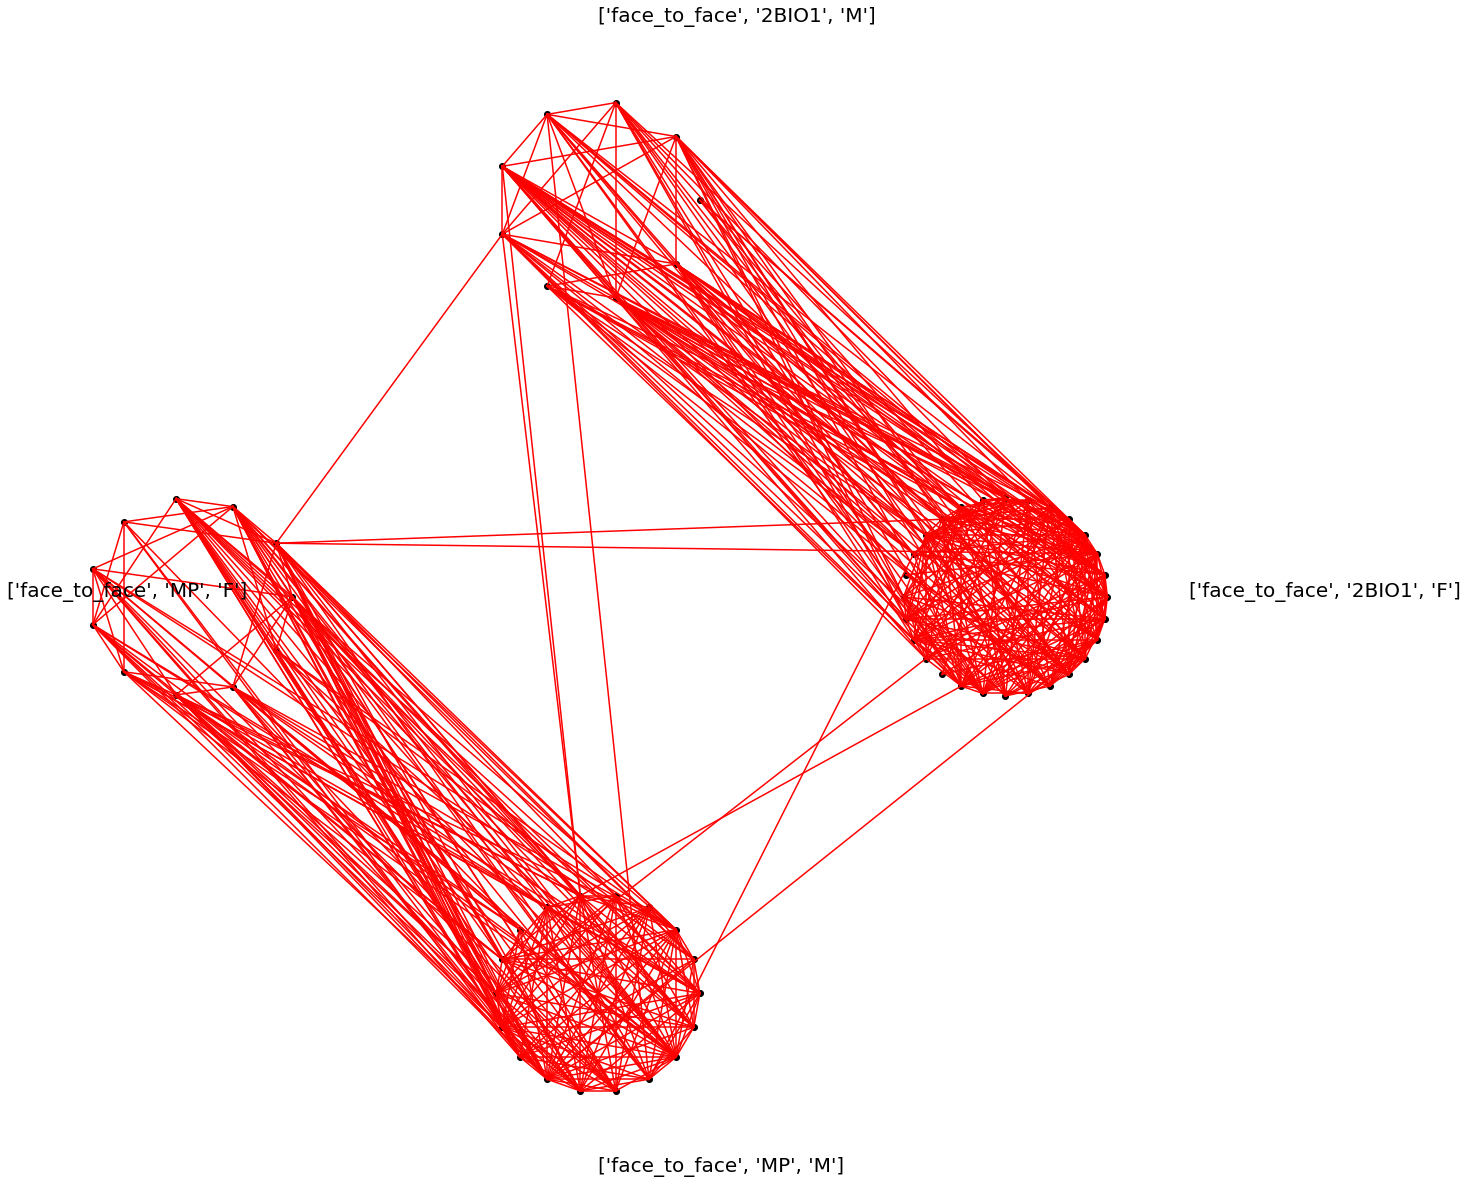
\includegraphics[width=\textwidth]{sousmulticlasseftf.png}
		\captionsetup{margin=10pt}
		\caption{\textbf{Visualisation du sous graphe induit multicouches des relations \texttt{'face to face'}, entre les élèves de deux classes} : les \texttt{'2BIO1'} et les \texttt{'MP'}.}
	\end{minipage}
	\label{induit}
	\caption{\textbf{Comparaison entre différents aspects du graphe multicouche. } On peut s'intéresser à la pertinence de séparer filles et garçons en différentes couches. En revanche, la séparation entre différentes classes semble être justifiée.}
\end{figure}


Nous avons donc calculé la densité des relations femmes/hommes comparée aux densité des relations au sein des hommes et des femmes.







\begin{figure}
	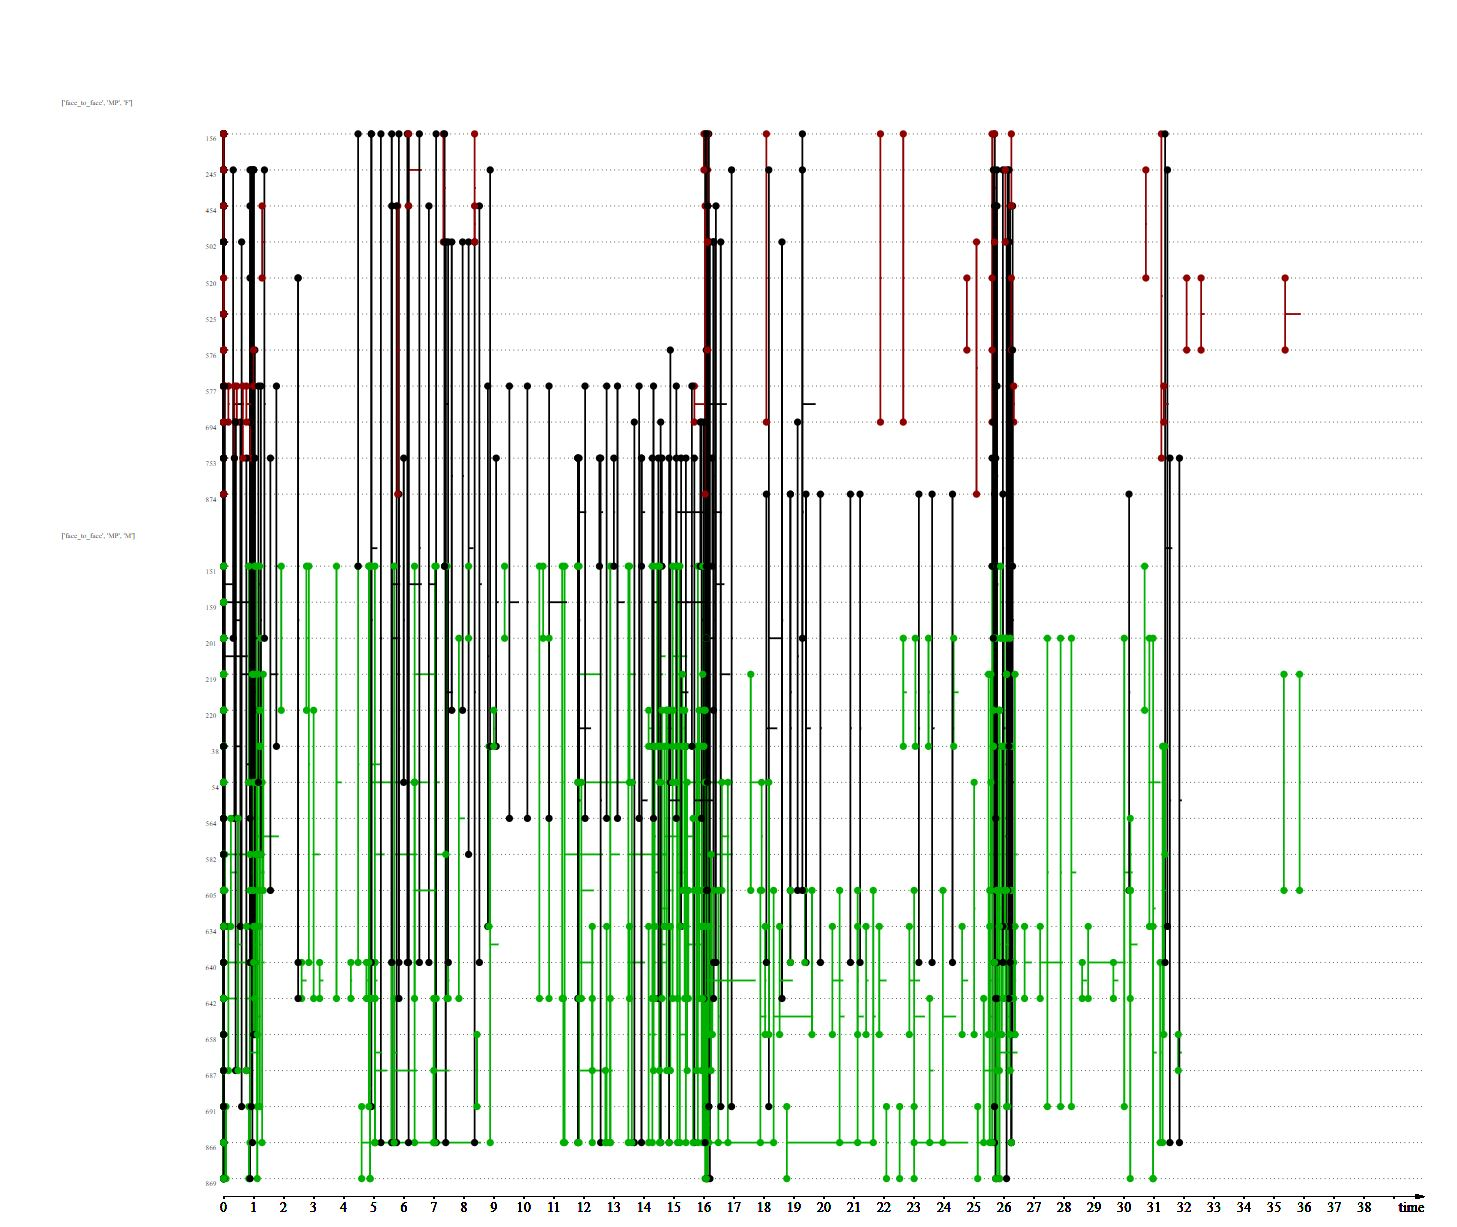
\includegraphics[width=\textwidth]{1jourMP.JPG}
	\caption{Une prise de vue le premier jour, des relations entre élèves féminins et masculins de la classe de MP. Nous y voyons "plus clair", cependant, il devient plus difficile de discerner les pauses.}
\end{figure}




\subsubsection{Densité : Repérer des "moments" importants}

\subsection{Star Wars}

Ce jeu de données recense toutes les scènes, les personnages et leurs scènes d'apparition, les dialogues, les mots-clés, les lieux.

Là encore, on peut représenter le graphe : 

\subsection{Avions ?}

\section{Conclusions et perspectives}

    \nocite{*}
    \bibliographystyle{plain}
	\bibliography{rapport}

\end{document}
